\documentclass[a4paper,11pt]{article}
\usepackage{hyperref}
\usepackage{graphicx}
\usepackage{url}
\usepackage{underscore}
\usepackage{float}

% Title Page
\title{IS project using Tensorflow with Keras}
\author{Razvan Pasca}


\begin{document}
\maketitle



\tableofcontents
\newpage
\section{Overview}
 
 \subsection{Running instructions}
 This installation steps refer to the Ubuntu x64 based version of the
 software, running on a CUDA Nvidia GPU. Everything was done according
 to the guide on the official site \cite{tensorflowSite}
   \subsubsection{Setting up python with anaconda on a fresh Ubuntu installation}
   \begin{enumerate}
   	\item curl -O \url {https://repo.continuum.io/archive/Anaconda3-5.0.1-Linux-x86_64.sh}	into a folder of your choice
   	\item bash Anaconda3-5.0.1-Linux-x86_64.sh
	\item Agree with license
   	\item Agree with env path updates
   	\item source ~/.bashrc
   	\item Check the install with conda command
	\item You can now create environments for the installation
   \end{enumerate}
   Q:What are python environments?\newline
   A:\url{https://realpython.com/python-virtual-environments-a-primer/}
	 
	\subsubsection{Installing Nvidia dependencies}
	First, to avoid wasting time: tensorflow says on its site that it
	supports CUDA toolkit 9.0. The link they provide redirects to toolkit
	9.1, which doesn’t work yet as it should. Don’t download from that
	link, but search manually where to get toolkit 9.0 or access
	 \url{https://developer.nvidia.com/cuda-90-download-archive}​ :)Also, I went for the runfile installation since getting it from the repo
	automatically takes the most recent version, 9.1, which we don’t want.
	Now, installation steps:
	\begin{enumerate}
		\item  sudo sh cuda_9.0.176_384.81_linux.run
		\item Follow instructions
		\item If the driver is not installed, that’s because you already have on
		running and need to disable it. If it’s version 384+ you should be fine,
		else see chapter V for extra info
	\end{enumerate}

	For CUDNN library, after creating an account on
	\url{https://developer.nvidia.com/cudnn}​ and downloading your desired version
	\begin{enumerate}
		\item sudo dpkg -i libcudnn7_7.0.3.11-1+cuda9.0_amd64.deb
		\item sudo dpkg -i libcudnn7-dev_7.0.3.11-1+cuda9.0_amd64.deb
		\item sudo dpkg -i libcudnn7-doc_7.0.3.11-1+cuda9.0_amd64.deb
	\end{enumerate}
	For libcupti-dev library, just do sudo apt-get install libcupti-dev and you are
	good to go.
	For more see \cite{cuddnGuide} and \cite{cuddnLinux}	
 
	\subsubsection{Installing Tensorflow and Keras with anaconda}
	To install the Tensorflow framework with anaconda the following steps should be enough
	\begin{enumerate}
		\item conda create -n tensorflow pip python=2.7 or python=3.3, etc.
		\item source activate tensorflow activates the environment to install
		tensorflow which will be called tensorflow
		\item pip install --ignore-installed --upgrade tfBinaryURL, taken from \cite{tensorflowBinary}
		\item pip install keras. By default, Keras uses Tensorflow as its default backend.
	\end{enumerate}

\subsection{Why Tensorflow?}
 TensorFlow is an interface for expressing machine learning algorithms, and an implementation for executing such algorithms. A computation expressed using TensorFlow can be executed with little or no change on a wide variety of heterogeneous systems, ranging from mobile devices such as phones and tablets up to large-scale distributed systems of hundreds of machines and thousands of computational devices such as GPU cards. The system is flexible and can be used to express a wide variety of algorithms, including training and inference algorithms for deep neural network models, and it has been used for conducting research and for deploying machine learning systems into production across more than a dozen areas of computer science and other fields, including speech recognition, computer vision, robotics, information retrieval, natural language processing, geographic information extraction, and computational drug discovery.\cite{tensorflowAbstract}] 
 
 When it comes to machine learning, it is easy to focus on the tech (features, capabilities, benchmarks, etc). But good programmers know it is much harder to write code that humans will use, versus code that a machine can compile and execute. Another important aspect about TensorFlow is the simple fact that everyone in the machine learning community is aware of it, most are open to trying it.
 
 \begin{figure}[H]
 	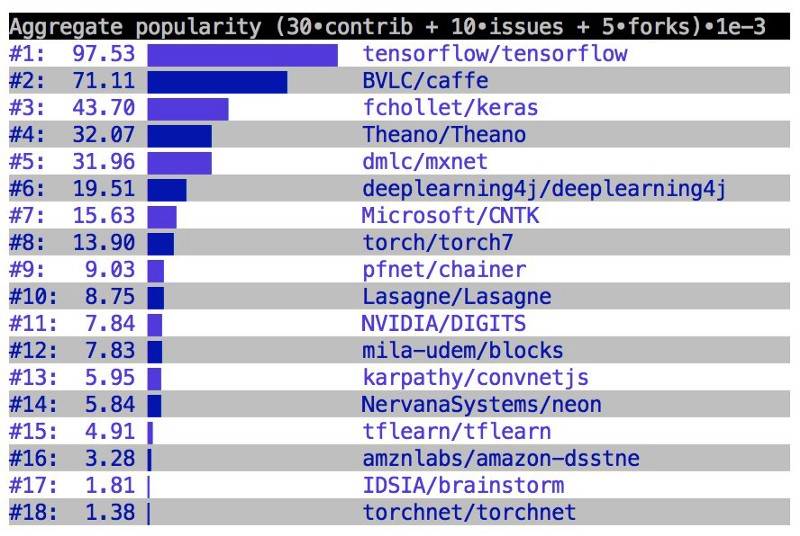
\includegraphics[width=\textwidth]{tensorflowPopularity.jpeg}
 	\caption{Popularity of different DL frameworks}
 \end{figure}
 
 A large number of developers and students are now interested in deep learning because they heard about TensorFlow. Google Deepmind recently announced they’ll be migrating from Torch to TensorFlow, so we might see an uptick in TensorFlow reinforcement learning models being released in the near future, too. The future is bright when the community embraces openness, clean APIs, useful modules, and the attitude of being helpful on the internet.
 
 \subsection{Theoretical aspects}
  \subsubsection{Data representation}
	It is known that having reliable datasets is very important for machine learning applications. In case of deep learning, some would say that it is more important than the algorithm, since having a lot of data allows the algorithms to learn more advanced features which in turn improve the performance and the developer to spend less time engineering features.
	\begin{figure}[H]
		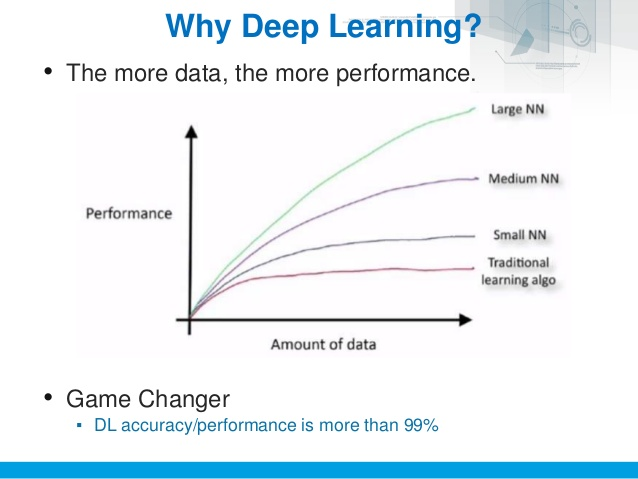
\includegraphics[width=\textwidth]{performanceComparison.jpg}
		\caption{performance of ML techniques as a function of amount of data}
	\end{figure}
	Therefore, 2 datasets have been considered for our application: The CIFAR dataset\cite{CIFAR} and a new dataset curated by Horea Muresan and Mihai Oltean. \cite{HoreaDataset} 
	These contain 60000 and 29000 images, with lots of categories, ranging from fruits to trucks and airplanes.
  \subsubsection{Algorithm}
	For this application a convolutional neural network approach is taken. Such a network
	can be composed of convolutional layers, pooling layers, ReLU layers, fully
	connected layers and loss layers. Convolutional layers consist of groups of neurons that make up kernels.
	The kernels have a small size but they always have the same depth as the
	input. The neurons from a kernel have a small receptive field, because it is
	highly inefficient to link all neurons to all previous outputs in the case of
	inputs of high dimensions such as images. Instead of each neuron having
	weights for the full dimension of the input, a neuron holds weights for the
	dimension of the kernel input. The kernels slide across the width and height
	of the input and produce a 2 dimensional activation map. 
	\begin{figure}[H]
		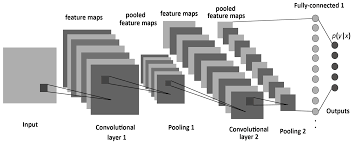
\includegraphics[width = \textwidth]{convo.png}
		\caption{Structure of a CNN}
	\end{figure}


	The stride at which a kernel slides is given as a parameter. The output of a convolutional
	layer is made by stacking the resulted activation maps.
	Pooling layers are used on one hand to reduce the spatial dimensions of
	the representation and to reduce the amount of computation done in the
	network. The other use of pooling layers is to control overfitting. The most
	used pooling layer has filters of size 2 x 2 with a stride 2. This effectively
	reduces the input to a quarter of its original size. ReLU layer, or Rectified
	Linear Units layer, applies the activation function max(0, x).It does not
	reduce the size of the network, but it increases its nonlinear properties.
	\begin{figure}[H]
		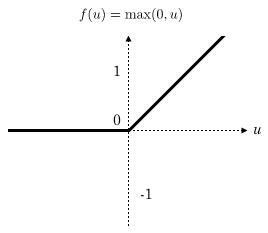
\includegraphics[width = 0.5\textwidth]{relu.png}
		\caption{Relu Function}
	\end{figure}

	Fully connected layers are layers from a regular neural network. Each neuron from
	a fully connected layer is linked to each output of the previous layer. The
	operations behind a convolutional layer are the same as in a fully connected
	layer. Thus, it is possible to convert between the two.
	Loss layers are used to penalize the network for deviating from the
	expected output. This is normally the last layer of the network. Various loss
	function exist: softmax is used for predicting a class from multiple disjunct
	classes, sigmoid cross-entropy is used for predicting multiple independent
	probabilities (from the [0, 1] interval). The input that we used consists of
	standard RGB images of size 100 x 100 pixels. The neural network that we
	used in this project has the structure given in Table 2.
	
	\subsubsection{Residual Networks}
	Experiments showed that the number of layers (depth) in a CNN is correlated to the performance in image recognition tasks. This led to the idea that deeper networks should perform better. Creating deep networks is not as simple as adding layers. One problem is the vanishing/exploding gradients, which hamper the convergence. This obstacle can be overcome by normalized initialization and intermediate normalization layers, so that networks start converging for stochastic gradient descend (SGD) using the backpropagation algorithm. Another problem is the degradation, if the depth of a network increases, the accuracy gets saturated and then degrades rapidly. A way to counter the degradation problem is using residual learning.\cite{resnet}
	\begin{figure}[H]
		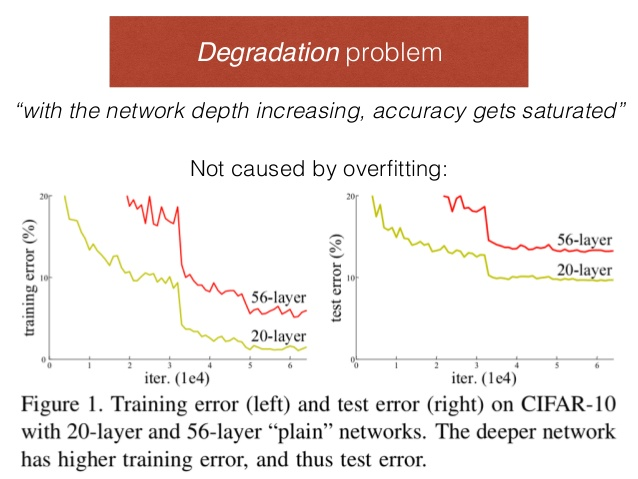
\includegraphics[width = \textwidth]{degradation.jpg}
		\caption{Degradation of performance}
	\end{figure}
	 
	 It is possible to fit an desired underlying mapping H(x)
	 by a few stacked nonlinear layers, so they can also fit an another underlying mapping F(x)=H(x)−x. As a result, it is possible to reformulate it to H(x)=F(x)+x, which consists of the Residual Function F(x) and input x. The connection of the input to the output is called a skipped connection or identity mapping. The general idea is that if multiple nonlinear layers can approximate the complicated function H(x), then it is possible for them to approximate the residual function F(x). Therefore the stacked layers are not used to fit H(x), instead these layers approximate the residual function F(x)
	 Both forms should be able to fit the underlying mapping.
	 One reason for the degradation problem could be the difficulties in approximating identity mappings by nonlinear layers. The reformulation used identity mapping as a reference and let the residual function represent the perturbations. The identity mapping can be generated by the solver through driving the weights of the residual function to zero if need be. 
	 
	 \begin{figure}[H]
	 	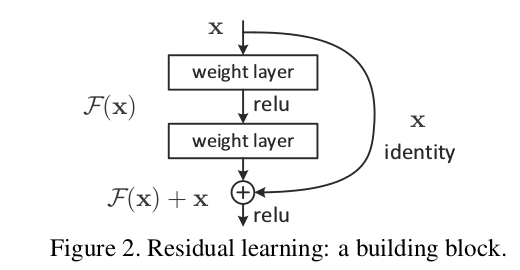
\includegraphics[width = \textwidth]{resnet.png}
	 	\caption{Resnet Module}
	 \end{figure}
	 
	 Residual learning is implemented to every few stacked layers. Figure 5 shows an example of 2 layers. As an example, formulation (1) can be defined as:
	 
	                             F(x)=W2σ(W1x)+x
	 
	 
	 Where W1 and W2 are the weights for the convolutinoal layers and σ is the activation function, in this case a RELU function. The operation F+x is realized by a shortcut connection and element-wise addition. The addition is followed by an activation function σ. The resulting formulation for a residual block is:
	 
	                                y(x)=σ(W2σ(W1x)+x)
	 
 \subsection{Existing Example}
	 One existing example which clearly shows the potential of the architecture is stated in the \cite{resnet}. It has achieved a performance of 3.57\% on the ImageNet test in 2015. The model has been trained on 1.28 million images and evaluated on 50k images. The objective was to correctly predict the class of an image according to a set of 1000 classes. The following output has been observed, comparing the accuracy with other well known architectures such as VGG and Inception. 
	 \begin{figure}[H]
	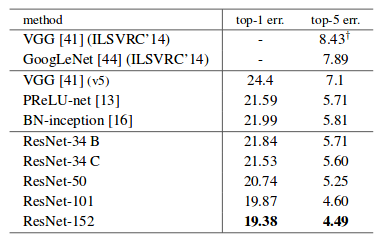
\includegraphics[width = \textwidth]{resnetError.png}
	\caption{Comparison between different architectures}
	 \end{figure}
	 

 \subsection{Your own small Example}
	In order to get more familiarized with the ResNet architecture, a small proof of concept module was developed. The scope of the app was to be able to distinguish between different digit signs made by hand, like the following:
	\begin{figure}[H]
		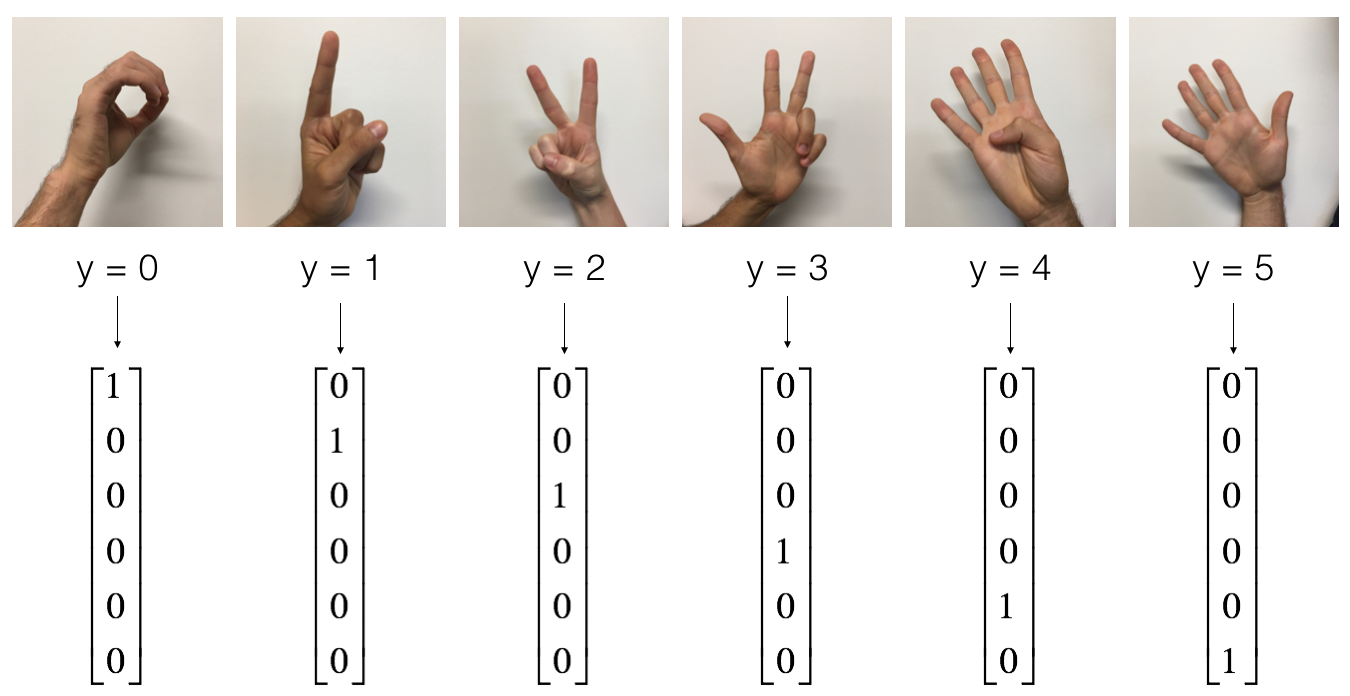
\includegraphics[width = \textwidth]{signs.png}
		\caption{Signs dataset}
	\end{figure}
    
    We have employed the following architecture, known as ResNet50, since it employs a residual learning architecture and a number of 50 layers. There are also versions of 100 and 152 layers, but for our task, 50 layers are more than enough. The following results have been obtained, after training the model for 20 epochs, on a batch size of 32.
    \begin{figure}[H]
    	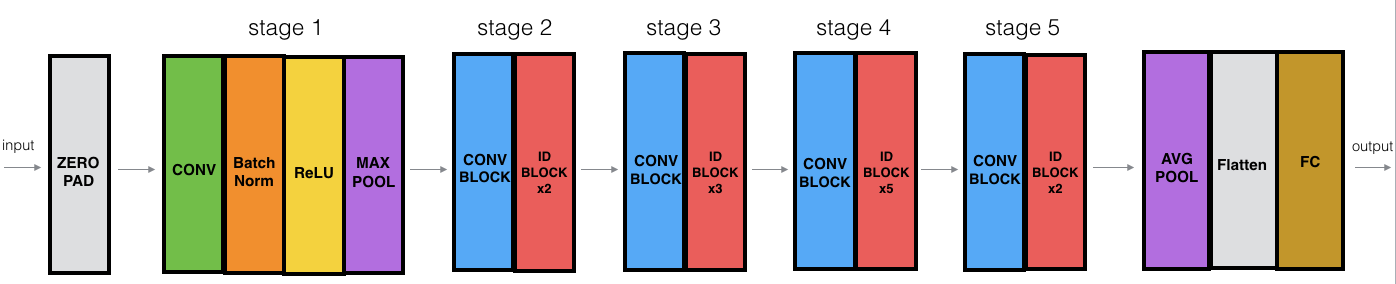
\includegraphics[width = \textwidth]{resnet50.png}
    	\caption{Resnet50 Architecture}
    \end{figure}
    
    \begin{figure}[H]
    	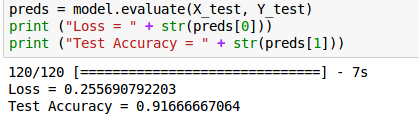
\includegraphics[width = \textwidth]{resnet50Acc.png}
    	\caption{Resnet50 Accuracy}
    \end{figure}

 \newpage
 \section{Proposed problem}
  \subsection{Specification} 
	The proposed application aims to solve the following problem as part of a larger IoT system. The final product is called Fridge.IO, an add-on for fridges which greatly increases the capabilities of such devices, by helping with keeping track of aliments inside, their expiration date and potential recipes which can be done with the contents, suggesting places to buy the missing ones. 
	
	One challenge with the system is automatizing the process of identifying the contents of the fridge and keeping track of inserted and removed aliments. For this part, a solution based on object identification has been proposed that should detect a range of classes of specific aliments
	\begin{itemize}
		\item Common fruits and vegetables
		\item Different types of meat and related products
		\item Beverages
		\item Home made aliments, if possible
	\end{itemize}
	 The images are going to be captured using a specialized webcam which is going to be placed either inside the fridge or outside, depending on the technical possibilities and the final hardware design. The final objective is to offer a fairly accurate overview of the fridge contents, offering the user the option to correct wrong predictions or to add his own aliments. Eventually, a shared classifier between the users will be made, and the images captured by the camera are going to be used as a future train set for different updates of the system.
	 
	 A beta version of the system can be checked at \url{http://iftp.avramiancuturda.ro/}. Currently, a basic database of aliments has been developed along an OCR for identifying the aliments from receipts. The mobile app is also available together with the web dashboard.
  
  
  \subsection{Implementation}
  
	  The final solution implementation has been carried out in the Tensorflow framework. The final architecture is shown in the following images, starting with an overview and zooming in the actual residual units. However, before going for this one, experiments with different variations and architectures have been made: InceptionV3, ResNetV1, ResNetV2
	  and Inception-ResNet. The development framework
	  used was Tensorflow together with Tensorflow
	  Hub \cite{tensorflowHub} for faster prototyping and model testing. The
	  models have been previously trained on the ImageNet
	  dataset \cite{imagenet}. 
	\newline

	  Using transfer learning, they have been
	  adapted for a different dataset consisting of various
	  fruits, namely Fruits-360 [20] for prototyping. The
	  models’ performance on the above datasets is presented
	  in Table 1. The Fruits-360 dataset has been adopted to
	  our case, giving up some more exotic fruit classes since
	  the computation capabilities were limited, reducing the
	  training time by 50\%. Moreover, the image sets has
	  been augmented, with 10\% of the images being picked
	  to be either cropped, zoomed in or flipped around one
	  of the axis, in order to increase the datasets’ variation.
	  The models were trained for 1000 steps on a corpus of
	  13.000 images, with 20\% of the pictures in the testing
	  set. Because of the reduced computing capabilities of our system, the final version contains 50 layers for feature extraction. A more detailed view is presented in Figures 11,12,13. The comparative performance of the models can be seen in the following table.

\begin{table*}[!h]
	\centering
	\begin{tabular}{ |c|c|c|c| } 
		\hline
		Model & ImageNet top-5 error & Fruits-360 Train accuracy & Fruits-360 Test accuracy \\
		\hline 
		Inception & 3.58\% & 98.0\% & 97.0\%\\ 
		ResNet v1 & 3.57\% & 99.0\% & 98.0\% \\ 
		ResNet v2 & 4.62\% & 99.0\% & 98.0\% \\ 
		Inception- ResNet & 3.08\% & 98.0\% & 98.0\%\\
		\hline
	\end{tabular}
	\newline
	\caption{Models' performance}
\end{table*}
	
	\begin{figure}[H]
		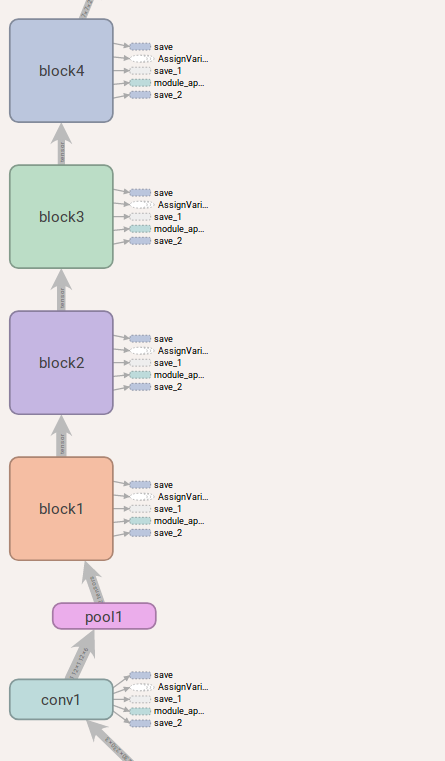
\includegraphics[height=3in]{modelabove.png}
		\caption{Top level architecture}
	\end{figure}
	
		
		\begin{figure}[H]
			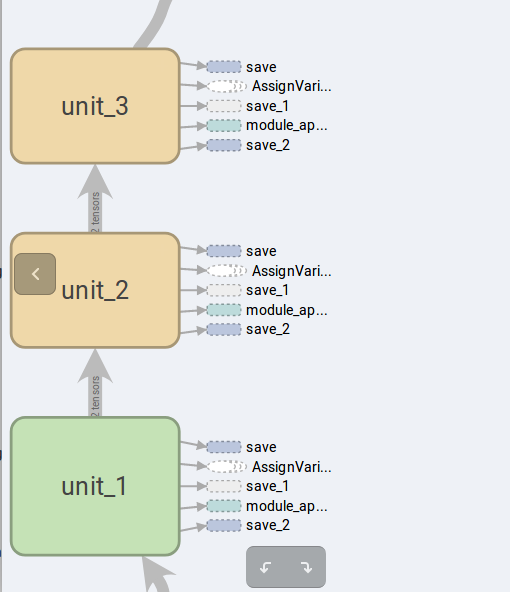
\includegraphics[height=3in]{blockarchitecture.png}
			\caption{Block architecture}
		\end{figure}
	
	In the following image, it can also be seen how the output of the previous unit enters 2 ways: one is processed by the next block and the other one goes uninterrupted and meets the other signal before the ReLu activation function is applied.

	\begin{figure}[H]
		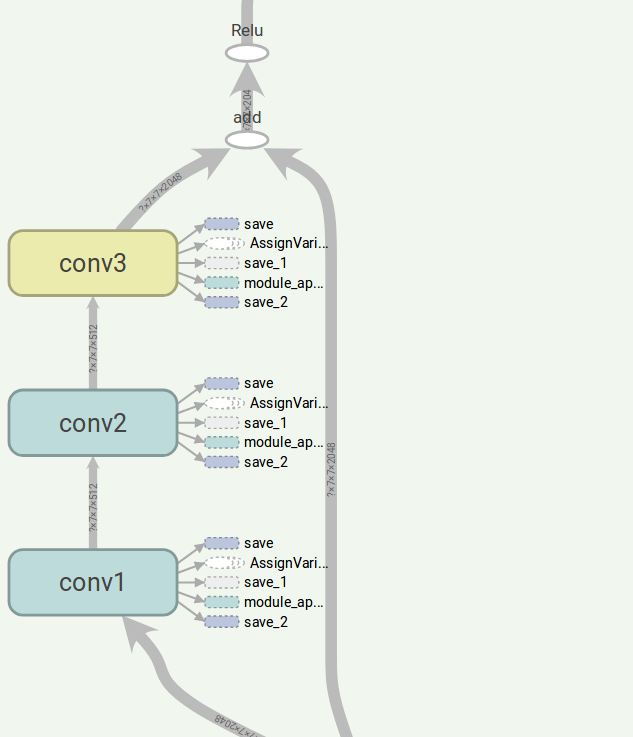
\includegraphics[height=3in]{resnetunit.png}
		\caption{Block architecture}
	\end{figure}

	  Given our use case, a single class detector would prove inefficient, since most of the time we present multiple aliments to the camera. Therefore, it should be able to detect multiple classes in the picture and choose the ones which have a higher confidence level. Therefore, the output node has been changed from a softmax layer which returns just the class with the highest probability to multiple sigmoid nodes which report their results independently from each other, something similar to Figure 14.
	  \newline
	  
	  This has proven effective but only for a reduced number of classes. Therefore, the amount of detected classes has been dropped from the initial 59 to just 3: apple, oranges and bananas. This allowed us to increase the performance on these classes by expanding the dataset using a webcralwer that downloaded images according to the given keywords. With that setup, the final loss looks like in Figure 15. The spikes in the curve are mostly owed to the different batches of images used for the training phase. Once the training was completed, the model was saved together with the weights for future use.
	  
	   \begin{figure}[H]
	   	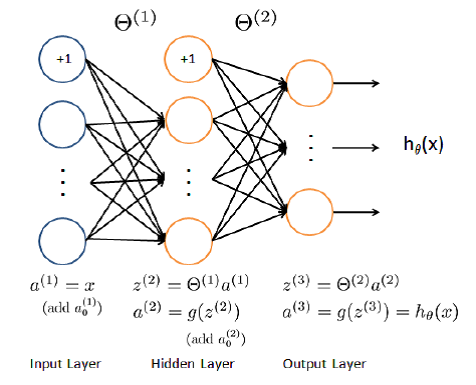
\includegraphics[height=3in]{multiclass.png}
	   	\caption{Multi class output}
	   \end{figure}
	  
	  	  
	  	  \begin{figure}[H]
	  	  	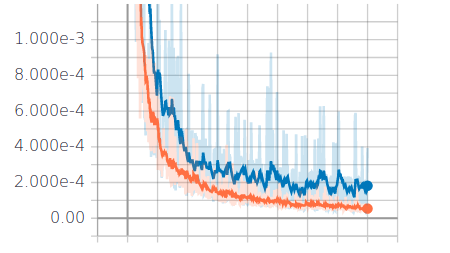
\includegraphics[height=2in]{loss.png}
	  	  	\caption{Final loss of the model}
	  	  \end{figure}

	  	
	  	The model is hosted on a Flask server written in Python using the Tensorflow serving api for sending images to the model and fetching predictions. The images come from a Raspberry Pi which takes pictures using a PiCam. The processing is done on the server, which updates the Firebase database accordingly. The whole system is hosted using Cloud services to ensure the system is permanently available. All the communication is done using HTTP requests, the image being encoded using base64 and the answers being provided in JSON form.The final architecture is similar to the one presented in Figure 16.
	  	 \begin{figure}[H]
	  	 	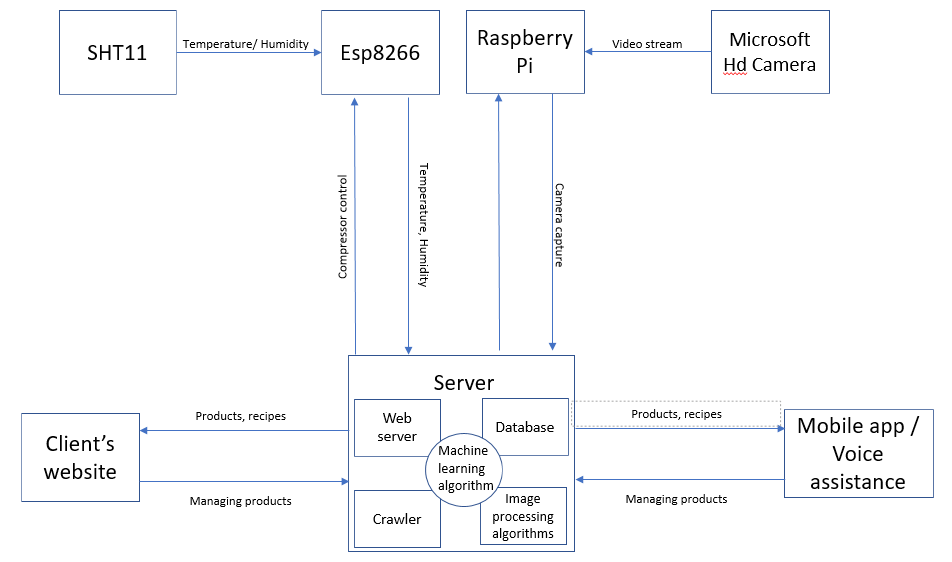
\includegraphics[height=3in, width=\textwidth]{architecture.png}
	  	 	\caption{System Architecture}
	  	 \end{figure}
	  
	 
	   \subsection{Conclusions and results}
	   
	   After some fine tunning of the model, we have reached satisfiable performance levels on the classes included for classification and detection. The raspberry pi has been set to send the requests periodically, and the webcam placed inside the fridge with a large field of view. As long as the view has not been blocked by other object, the accuracy measured is over 90\%.
	   
	    The results are also updated as long as the network connection is reliable. For images which contain more instances of the same fruit, however, there are no means currently to "count" them, thus the performance is affected by this use case. Also, the system has proven to be reliable in low light settings or on noisy pictures thanks to the augmentation performed on the dataset.
	   
	   \subsubsection{Future improvements}
	   
	   The model used for image recognition can
	   be finely tuned or a more specific developed model can be
	   applied for the problem. This is especially due to the inability of the current system to count the number of presences of an object in an image. Therefore, a architecture specialized in object detection such as YOLO or R-CNN should prove more efficient. However, given the historic of
	   Deep Learning algorithms, the another big improvement can
	   be made by using a larger data set. This can be achieved
	   by collecting the pictures taken at user level together with
	   their feedback through the application and periodically
	   release new model updates. 
	   
	   Also, a more  ambitious approach would be to use more cameras and concatenate their pictures together in order to cover as many blind spots as possible. This would effectively allow to take more pictures from different positions and grab more information about the structure and contents of the fridge. In the end, the concatenated picture would be passed through a network tailored to work on this kind of images.
  
\newpage
\bibliography{References}
\bibliographystyle{plain}

\end{document}          
